\documentclass[12pt]{article}

\usepackage{amsmath}
\usepackage{unicode-math}
\usepackage{xltxtra}
\usepackage{xgreek}

\setmainfont{Liberation Serif}

\usepackage{tabularx}

\pagestyle{empty}

\usepackage{geometry}
 \geometry{a4paper, total={190mm,280mm}, left=10mm, top=10mm}

 \usepackage{graphicx}
 \graphicspath{ {images/} }

 \usepackage{wrapfig}
\usepackage{lipsum}%% a garbage package you don't need except to create examples.

\begin{document}

\section*{Θέμα Α}
  \noindent
  \begin{enumerate}
    \item \textbf{[Μονάδες 15]} Απόδειξη από το βιβλίο.
    \item \textbf{[Μονάδες 10]} Σ, Σ, Λ, Λ, Σ
  \end{enumerate}

\section*{Θέμα Β}
  \noindent
  \begin{wrapfigure}[4]{r}{0.3\textwidth}
    \centering
    \vspace{-140pt}
    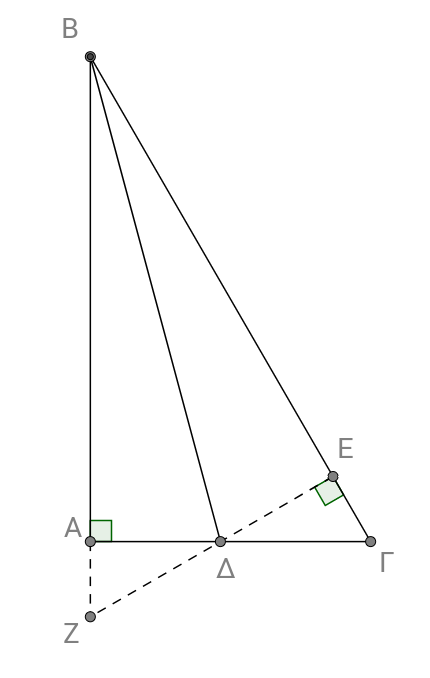
\includegraphics[width=0.3\textwidth]{2017AGeo2}
  \end{wrapfigure}
  \begin{enumerate}
    \item \textbf{[Μονάδες 10]} Συγκρίνουμε τα τρίγωνα $ΒΑΔ$ και $ΒΕΔ$ (ορθογώνια με υποτείνουσα και οξεία γωνία).
    \item \textbf{[Μονάδες 15]} Συγκρίνουμε τα τρίγωνα $ΔΑΖ$ και $ΔΕΓ$ (Γ-Π-Γ) $\implies ΑΖ=ΕΓ$. Από πριν $ΒΑ=ΒΕ$, άρα $ΒΖ=ΒΓ$.
  \end{enumerate}

\section*{Θέμα Γ}
  \noindent
  \begin{wrapfigure}[4]{r}{0.4\textwidth}
    \centering
    \vspace{-20pt}
    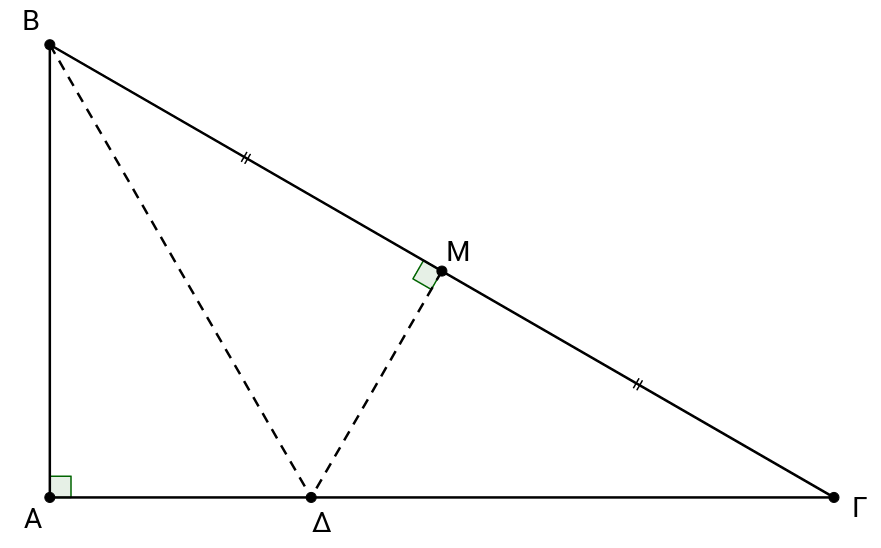
\includegraphics[width=0.4\textwidth]{2017AGeo3}
  \end{wrapfigure}
    \begin{enumerate}
    \item \textbf{[Μονάδες 8]} Αφού $ΜΔ$ μεσοκάθετος, $ΔΒ=ΔΓ$. Έτσι το τρίγωνο $ΒΔΓ$ είναι ισοσκελές με $\hat{Γ}=\widehat{ΜΒΔ}=30^{\circ}$. Η γωνία $Β$ είναι $60^{\circ}$ άρα διχοτομείται.
    \item \textbf{[Μονάδες 9]} Συγκρίνω τα τρίγωνα $ΒΑΔ$ και $ΒΜΔ$ (Ορθογώνια με υποτείνουσα και οξεία). Έτσι $ΑΔ=ΔΜ$. Αλλά $ΔΜ=\frac{ΔΓ}{2}$ ως πλευρά ορθογωνίου απέναντι από $30^{\circ}$. Έτσι $ΔΓ=2ΑΔ \implies ΔΜ=\frac{ΑΓ}{3}$.
    \item \textbf{[Μονάδες 8]} Οι διαγώνιοι διχοτομούνται κάθετα.
  \end{enumerate}

\section*{Θέμα Δ}
  \noindent
  \begin{wrapfigure}[4]{r}{0.4\textwidth}
    \centering
    \vspace{-50pt}
    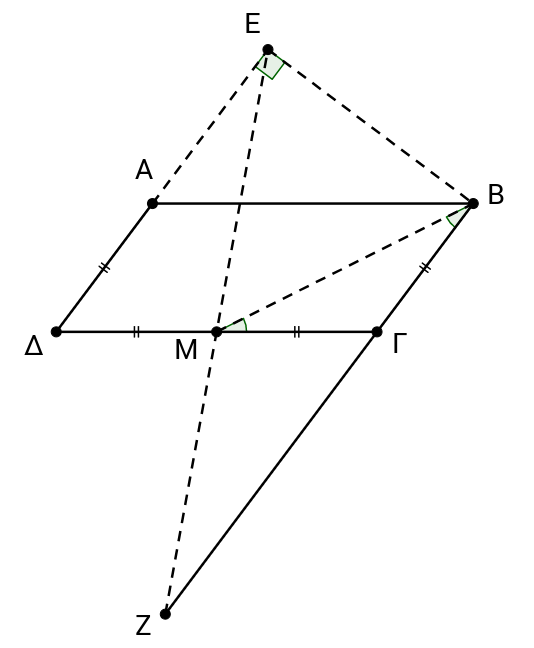
\includegraphics[width=0.4\textwidth]{2017AGeo4}
  \end{wrapfigure}
  \begin{enumerate}
    \item \textbf{[Μονάδες 5]}  $ΜΓ=ΒΓ$ άρα $ΜΒΓ$ ισοσκελές.
    \item \textbf{[Μονάδες 6]}  (Γ-Π-Γ με $Μ_1=Μ_2,ΔΜ=ΜΓ,Δ=Γ$).
    \item \textbf{[Μονάδες 5]}  Από πριν $Ε_1=Ζ$ και αφού $Ε=90^{\circ}$ θα ισχύει $E_2+Z=90^{\circ} \implies Β=90$.
    \item \textbf{[Μονάδες 6]}  Στο τρίγωνο $ΒΕΖ$, η $ΒΜ$ είναι διάμεσος που αντιστοιχεί στην υποτείνουσα άρα $ΒΜ=ΜΖ$.
    \item \textbf{[Μονάδες 3]}  Παραλληλόγραμμο με μία ορθή.
    \item \textbf{[Μονάδες 5]}  $Α$ μέσο $ΔΕ$ και $Μ$ μέσο $ΕΖ$. Το $ΑΜ$ είναι ευθύγραμμο τμήμα που ενώνει τα μέσα των δύο πλευρών.
  \end{enumerate}
\end{document}
